\section{Architecture}
% Reference 'Uwe08' and 'uweref' in sources folder.

In this section the architecture of the votes system is define. The viewpoints are taken from the UWE approach proposed in \cite{Uwe08,uweref} and use UML stereotypes. In the next sections the focus lies on the content, navigation and presentation model as the requirements are already define in \ref{requirements}.



\subsection{Content Model}
The following perspective describes the systems content model derived from requirement analysis model. The viewpoint is defined in \cite{Uwe08,uweref}, disregarding of the definition, the view is conform to a regular class diagram and does not use any stereotypes. Model elements for behaviour (like Operations) are not contained in this perspective.

The votes content model can be seen in figure \ref{content_model}. The corresponding implementation serves as backbone of the running application in form of keeping the data and persisting it on a database. Later this is realises by JPA. Importance comes to the fact that no presentation details are included in the model, only the domain knowledge is included. The six classes represent all essential entity types that are involved in the requirements and their corresponding properties. Two enumeration types serve as additional datatypes. 

High value comes to this view due to the fact that it can be directly mapped on the JPA and the transfer object classes that are part of the systems implementation. Apart from the fixed nature of the content model, described in the current requirements, a derivation process defining the Java classes can be of high good for further evolution and maintenance providing constructive quality assurance.

\begin{figure}
\centering
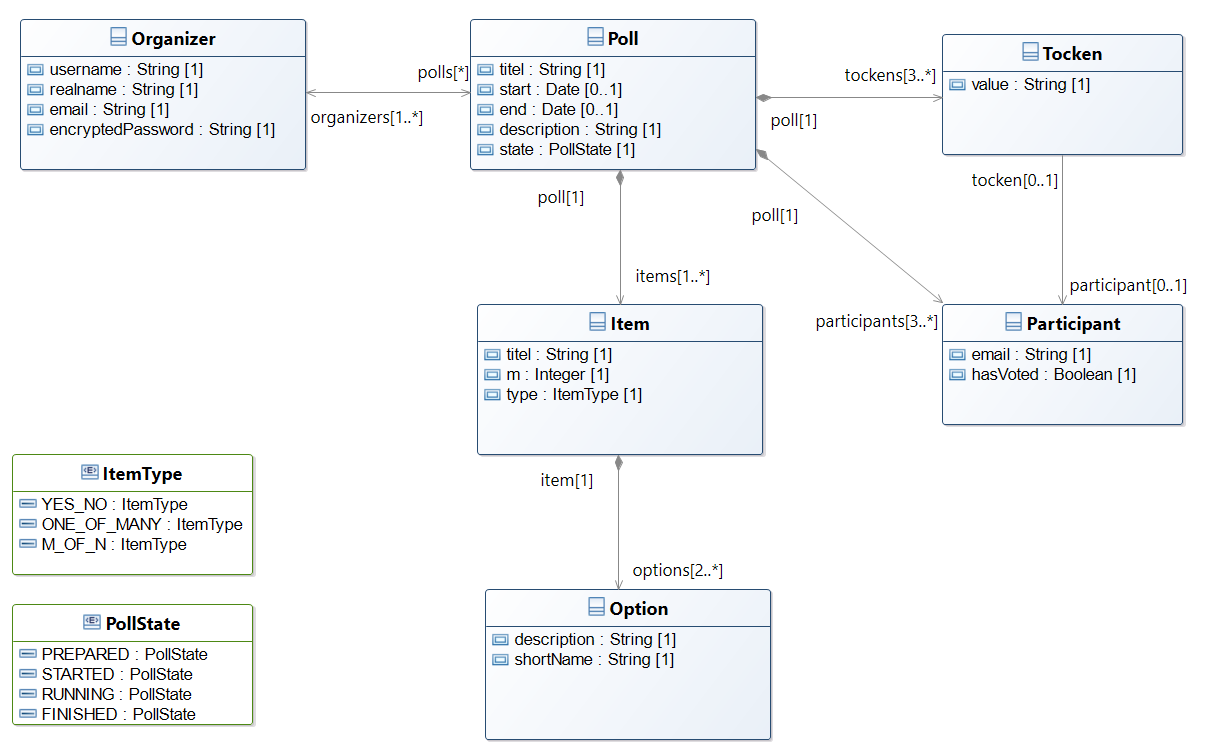
\includegraphics[width=1.0\textwidth]{png/domain_model.png}
\caption{Votes content model}
\label{F:content_model}
\end{figure}


\subsection{Navigation model}
% Max has to check the models that.
The navigation through the system and the interaction between user and content model is realised in html. The following model presented in figure \ref{F:navigation_model} focuses on the possible navigation paths. To define this on an abstract level we will coarsely stick to navigation model viewpoint defined by the UWE approve \cite{Uwe08,uweref}. It defines possible ways through the system by specifying different node types and one navigation links on the basis of UML stereotypes. A node is the smallest unit where any user can navigate to but more than one node can be presented on a single web page. Links are used to connect nodes and enable transitions, containment relations points out the structural containedness of one node in another.

\begin{figure}
\centering
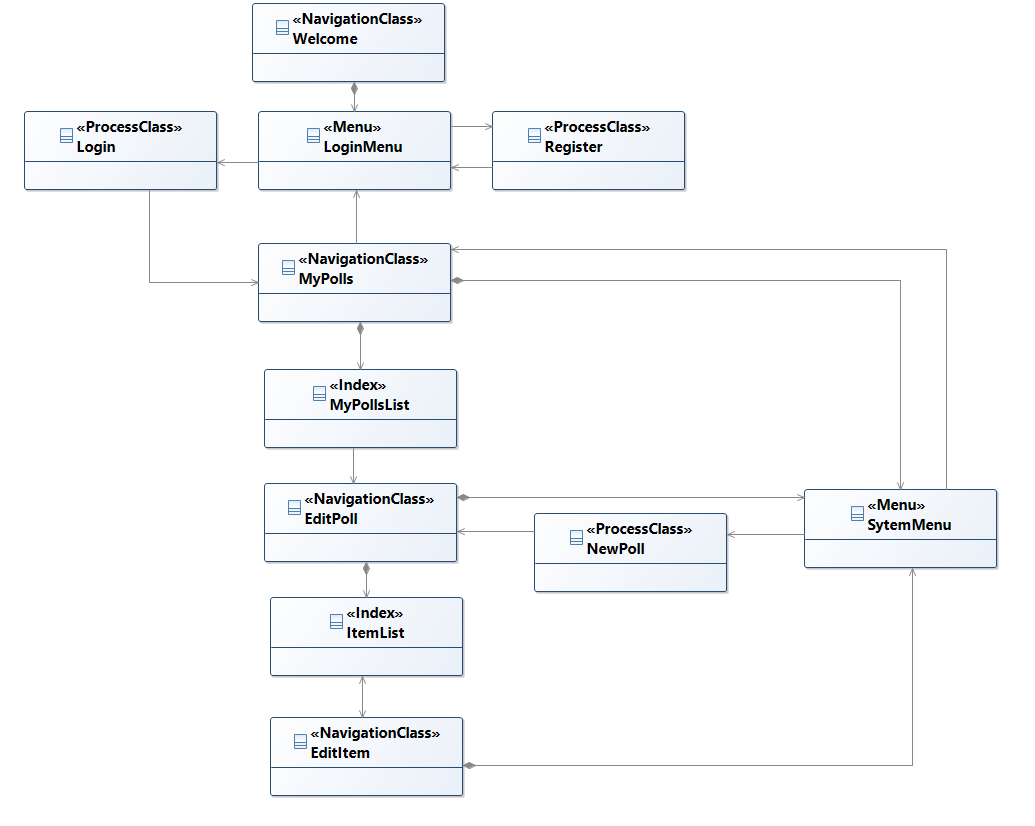
\includegraphics[width=1.0\textwidth]{png/navigation_model.png}
\caption{Votes navigation model}
\label{F:navigation_model}
\end{figure}

\subsection{Presentation model}
% If we insert the UWE Presentation model, i need help of max because i can not undesand html jsf.

The presentation model describes the components involved in the user interface and their relations. In the following model, displayed in figure \ref{F:presentation_model}, and its realisations web page, plotted in \ref{F:presentation_model_realisation}, the underlying structure is pointed out by using the example of the 'My Polls' page. The page consists of two parts and is defined by the component type MyPolls. The lower region holds one list displaying polls, the upper side displays the menu that allows the user to go back to the 'My Polls' page or to create a new Poll. In the case of the 'My Polls' type the left button of the SystemMenu part links back to the page itself. This is necessary because the SystemMenu type is also used in other context where it is needed to have a link back to the 'My Polls' page. Other pages of the votes system can be defined in similar fashion. The visual UWE stereotypes are missing in this model because of technical reasons.

 
\begin{figure}
\centering
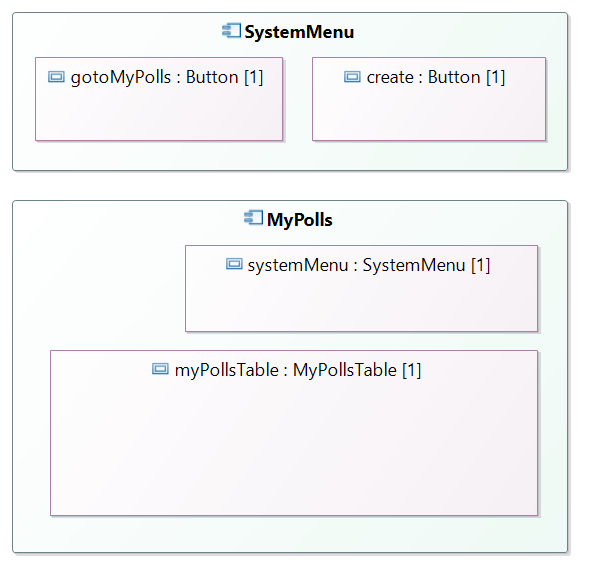
\includegraphics[width=0.4\textwidth]{png/presentation_model.png}
\caption{Votes presentation model of 'My Polls' page}
\label{F:presentation_model}
\end{figure}

\begin{figure}
\centering
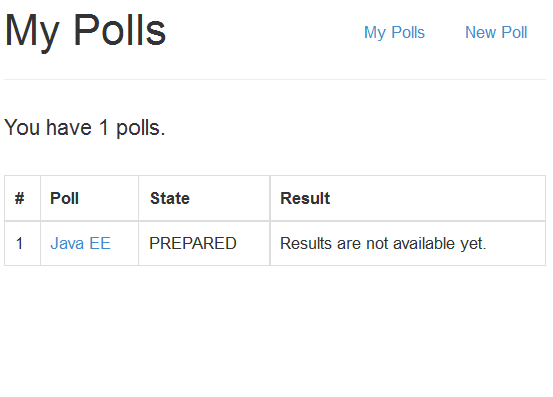
\includegraphics[width=0.4\textwidth]{png/presentation_model_realisation.png}
\caption{Votes realisation of 'My Polls' page}
\label{F:presentation_model_realisation}
\end{figure}

\subsection{VotesWar Architecture (Packaging?)}
% Do you mean packaging?